\documentclass[11pt,oneside,a4paper]{standalone}

\usepackage{mathtools}

\usepackage{tikz}
\usetikzlibrary{matrix}
\usetikzlibrary{arrows}

\DeclareMathOperator{\Coker}{Koker}
\DeclareMathOperator{\Ker}{Ker}

\begin{document}
  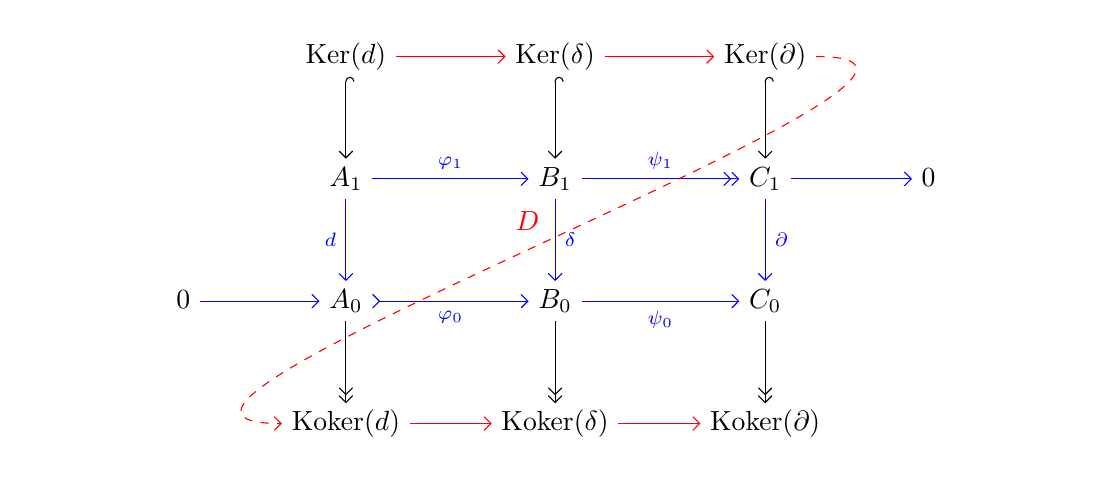
\begin{tikzpicture}[>=angle 90]
    \matrix[matrix of math nodes,
    row sep=3em, column sep=3em,,
    text height=1.5ex, text depth=0.25ex]
    {
      &&|[name=kd]| \Ker(d) & |[name=kdelta]| \Ker(\delta)
      &|[name=kdel]| \Ker(\partial) \\
      &&|[name=A1]| A_1 &|[name=B1]| B_1 &|[name=C1]| C_1 &|[name=01]| 0 \\
      &|[name=00]| 0 &|[name=A0]| A_0 &|[name=B0]| B_0 &|[name=C0]| C_0 \\
      &&|[name=cd]| \Coker(d) &|[name=cdelta]| \Coker(\delta) &|[name=cdel]|
      \Coker(\partial) \\
    };
    \draw[right hook->,font=\scriptsize]
          (kd) edge (A1)
          (kdelta) edge (B1)
          (kdel) edge (C1);
    \draw[>->,font=\scriptsize,blue]
          (A0) edge node[below] {$\varphi_0$} (B0);
    \draw[->>,font=\scriptsize,blue]
          (B1) edge node[auto] {$\psi_1$} (C1);
    \draw[->,font=\scriptsize,blue]
          (A1) edge node[auto] {$\varphi_1$} (B1)
          (B0) edge node[below] {$\psi_0$} (C0)
          (A1) edge node[left] {$d$} (A0)
          (B1) edge node[auto] {$\delta$} (B0)
          (C1) edge node[auto] {$\partial$} (C0)
          (C1) edge (01)
          (00) edge (A0);
    \draw[->>,font=\scriptsize]
          (A0) edge (cd)
          (B0) edge (cdelta)
          (C0) edge (cdel);
    \draw[->,red]
          (kd) edge (kdelta)
          (kdelta) edge (kdel)
          (cd) edge (cdelta)
          (cdelta) edge (cdel);
    \draw[->,dashed,red]
          (kdel) edge[out=0,in=180,red] node[above left] {$D$} (cd);
  \end{tikzpicture}
\end{document}